










\subsection{Earth-Sun system}








\subsubsection{Stability}

\begin{figure}[H]
    \centering
    \begin{subfigure}{0.5\textwidth}
        \centering
        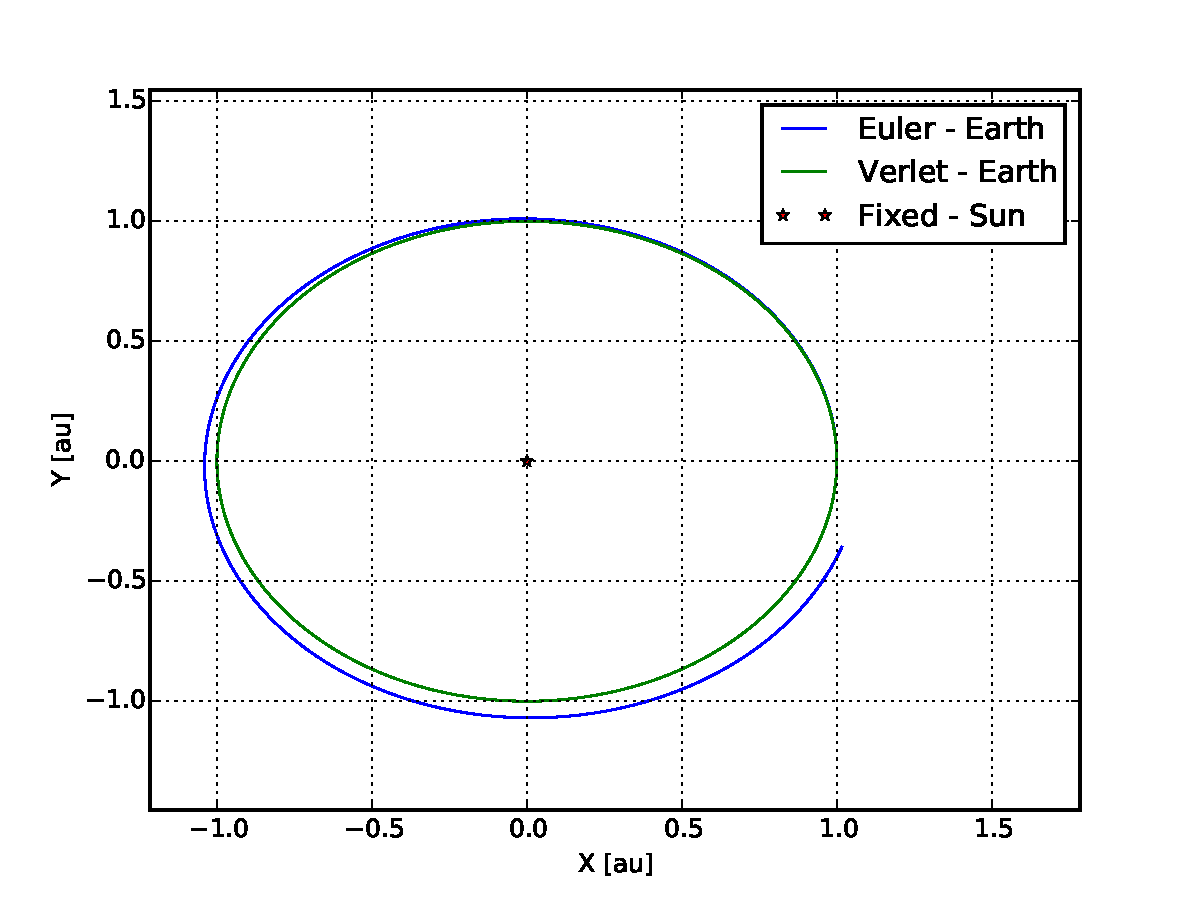
\includegraphics[width=\linewidth]{result/bilder/earth-sun.pdf}
    	\caption{}
    \end{subfigure}%
    ~ 
    \begin{subfigure}{0.5\textwidth}
        \centering
        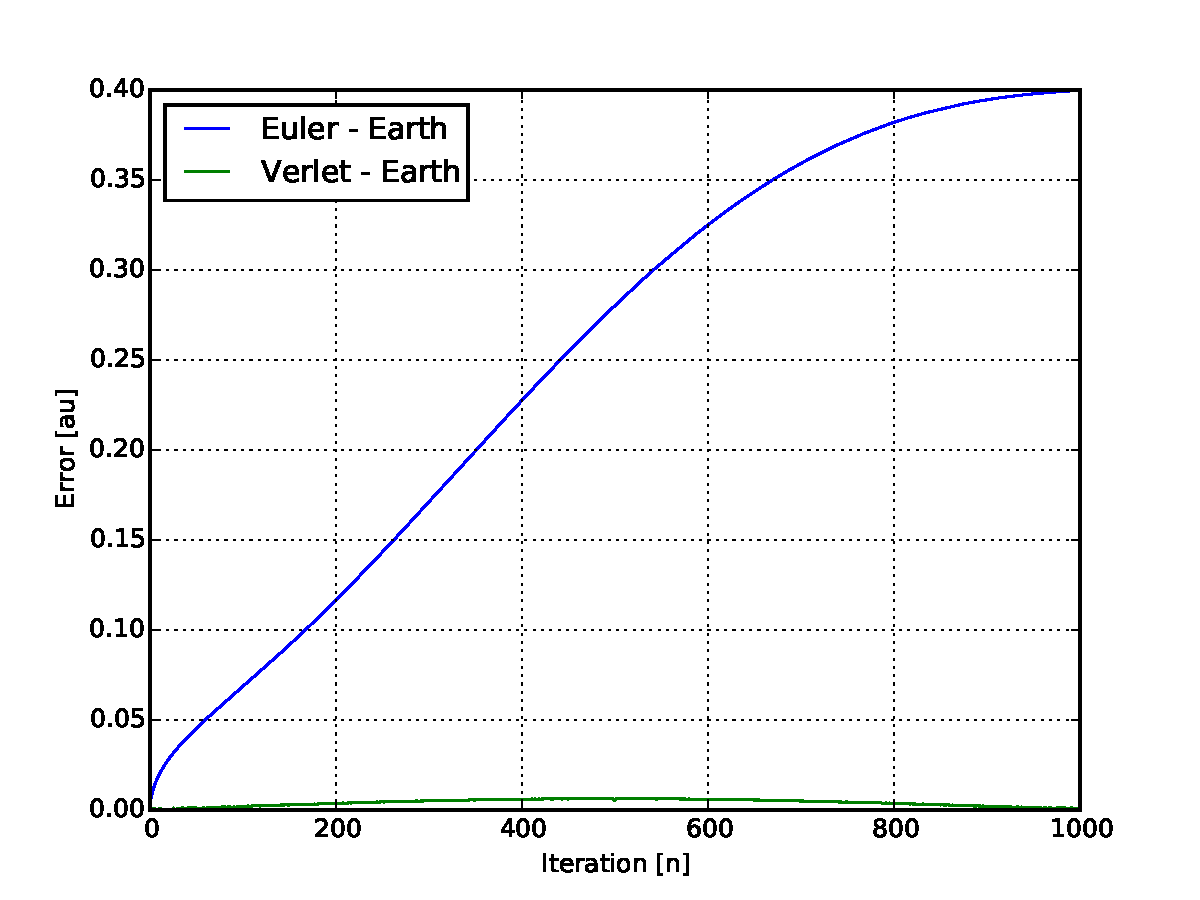
\includegraphics[width=\linewidth]{result/bilder/earth-sun-error.pdf}
        \caption{}
    \end{subfigure}
    \caption{a) shows the orbit of earth around the sun. The intial velocity is set to $2\pi$ in y direction and the start position to 1 au in x direction. b) shows how the error develops. The intial values should give a perfect circular motion. So the error is calculated by $r_i - r_{0}$. It is apparent that the Verlet-Velocity method is a better approximation. This simulation was with 1000 points with the end time of 1 year. Both simulations was produced by \href{https://github.com/erikfsk/Project-3/tree/master/Project3/earth-sun-standard-results}{\textcolor{blue}{plot\_earth\_sun.py}}}
    \label{fig:earth-sun}
\end{figure}


\begin{center}
\label{table:euler-verlet-time}
\captionof{table}{Time table for the different algorithms. The algorithms use nearly the same time. This is not a shocker since the number of FLOPs for the algorithms are similar, see section (\ref{sec:flops}). Note: this is only the result from one test, but several was done. Both algorithms were very close and it seems to be random which is fastest.
\\}
\begin{tabularx}{\textwidth}{c c c c c c c c}
    \hline 
    \hline 
    n & Forward-Euler & Verlet-Velocity &  fastest &&&& $\frac{slowest}{fastest}$\\ 
    \hline
    10 & 0.000136 & 0.000148 & Euler &&&&   1.08823529412   \\ 
    100 & 0.000208 & 0.000179 & Verlet &&&&   1.16201117318   \\ 
    1000 & 0.000392 & 0.000389 & Verlet &&&&  1.00771208226   \\ 
    10000 & 0.002427 & 0.002426 & Verlet &&&&   1.00041220115  \\ 
    100000 & 0.022931 & 0.022293 & Verlet &&&&   1.02861884897   \\ 
    1000000 & 0.167022 & 0.175944 & Euler &&&&   1.05341811258  \\ 
    10000000 & 1.58721 & 1.52666 & Verlet &&&&   1.03966174525  \\ 
    100000000 & 15.1786 & 15.1176 & Verlet &&&&   1.00403503202  \\ 
    \hline
\end{tabularx}
\end{center}














\subsubsection{Conserved quantities}

All the figures in this section was made from the data and python script in the directory \href{https://github.com/erikfsk/Project-3/tree/master/Project3/conserved-values}{\textcolor{blue}{conserved-values}}.

\begin{figure}[H]
    \centering
    \begin{subfigure}{0.5\textwidth}
        \centering
        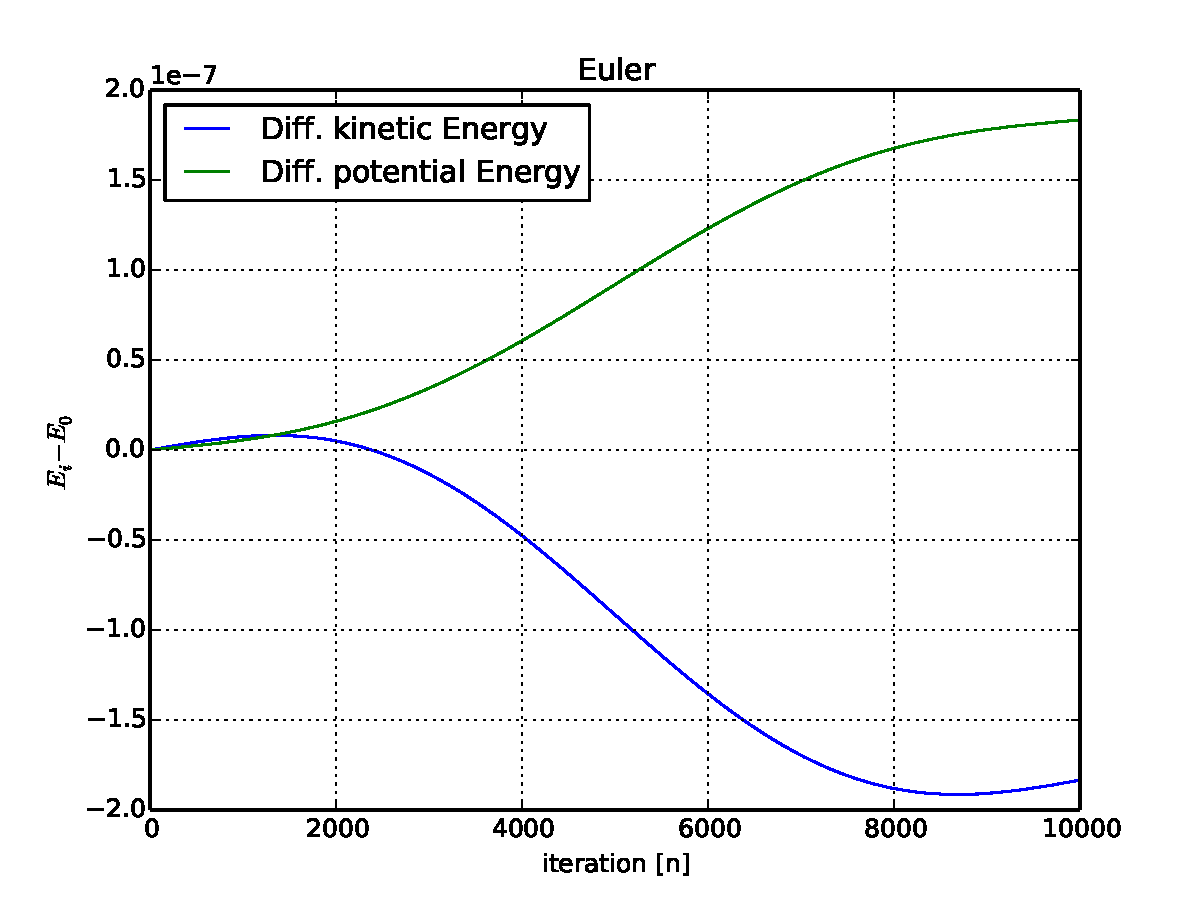
\includegraphics[width=\linewidth]{result/bilder/kin-pot-euler.pdf}
    	\caption{}
    \end{subfigure}%
    ~ 
    \begin{subfigure}{0.5\textwidth}
        \centering
        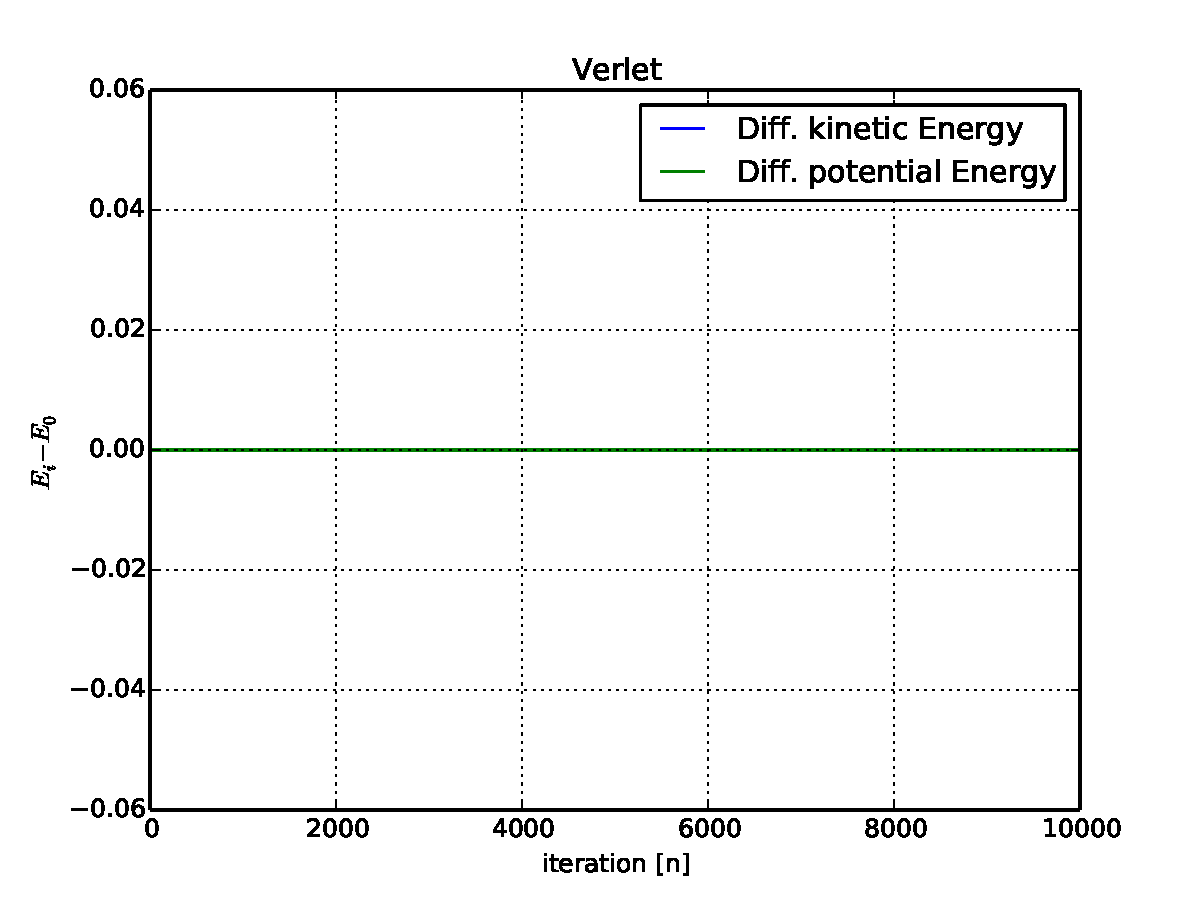
\includegraphics[width=\linewidth]{result/bilder/kin-pot-verlet.pdf}
        \caption{}
    \end{subfigure}
    \caption{The graphs show the change in kinetic and potential energies compared to their initial values a) is the Forward Euler method and b) is the Verlet-Velocity method.}
    \label{fig:conserved-energy}
\end{figure}

 As expected the energies are not conserved in the Forward Euler method, but is conserved in the Verlet-Velocity.



\begin{figure}[H]
    \centering
    \begin{subfigure}{0.5\textwidth}
        \centering
        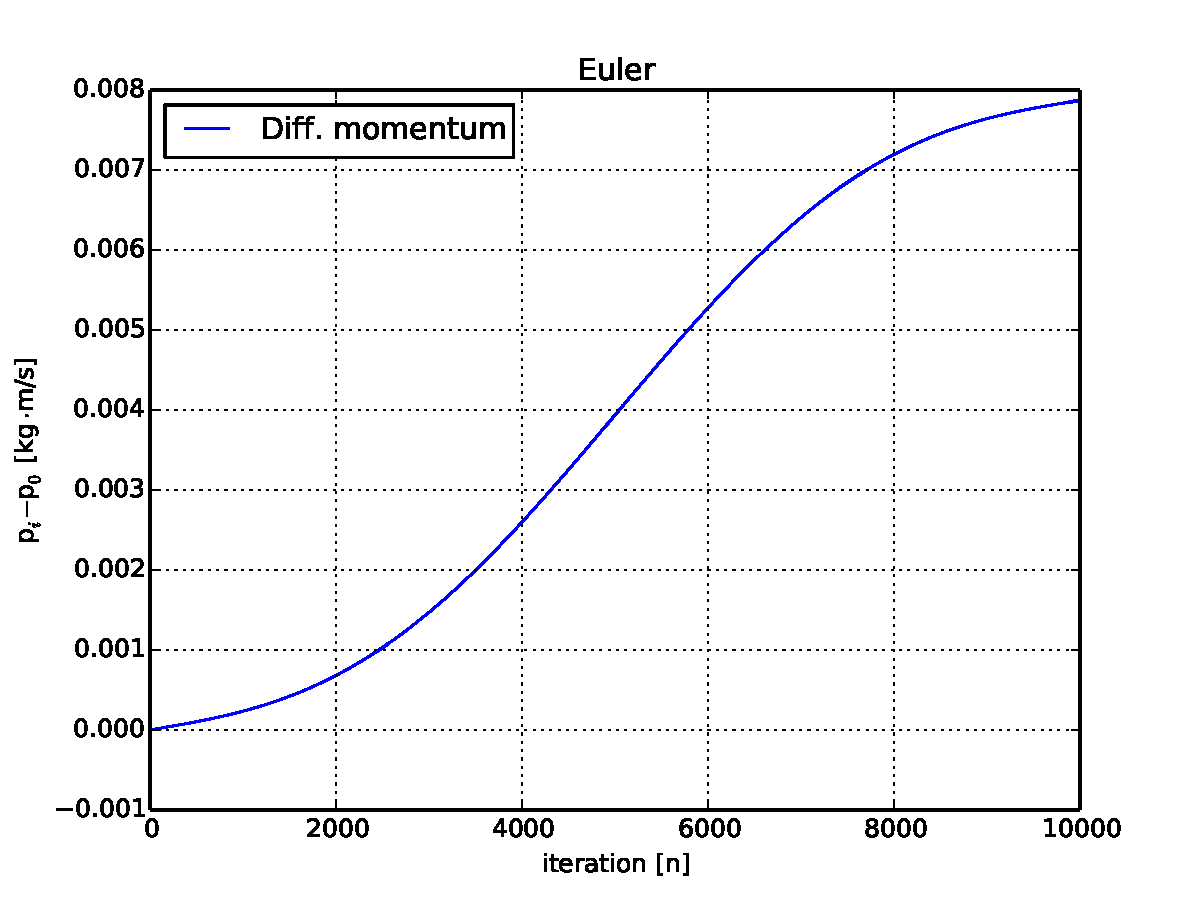
\includegraphics[width=\linewidth]{result/bilder/momentum-euler.pdf}
    	\caption{}
    \end{subfigure}%
    ~ 
    \begin{subfigure}{0.5\textwidth}
        \centering
        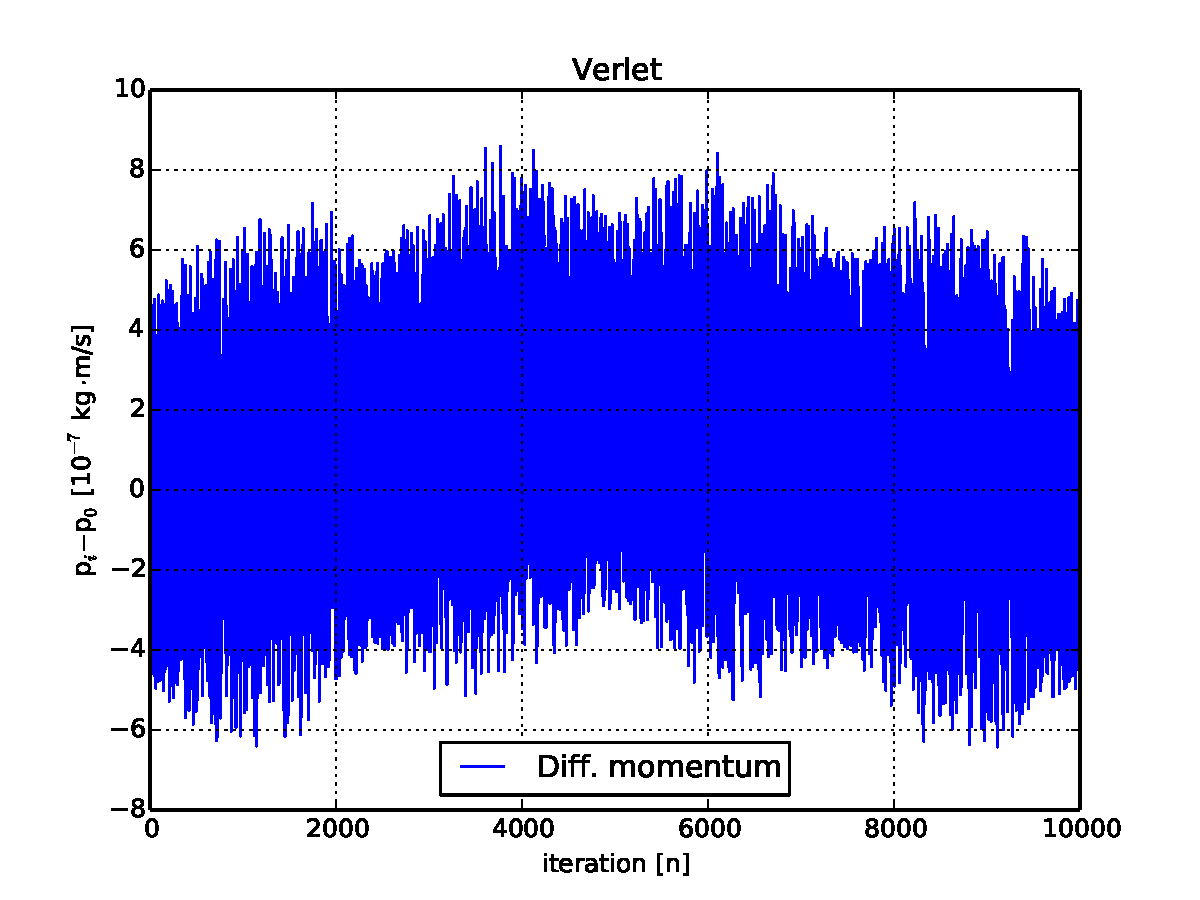
\includegraphics[width=\linewidth]{result/bilder/momentum-verlet.pdf}
        \caption{}
    \end{subfigure}
    \caption{Both graphs are of the momentum and how they differ from their intial values. a) is the Forward Euler method and b) is the Verlet-Velocity method.
    }
    \label{fig:conserved-momentum}
\end{figure}

 It should come as no suprise that momentum is not conserved for the Forward Euler method as the kinetic energy was not conserved. Once again the Verlet-velocity method conserves the quantity. 



\begin{figure}[H]
    \centering
    \begin{subfigure}{0.5\textwidth}
        \centering
        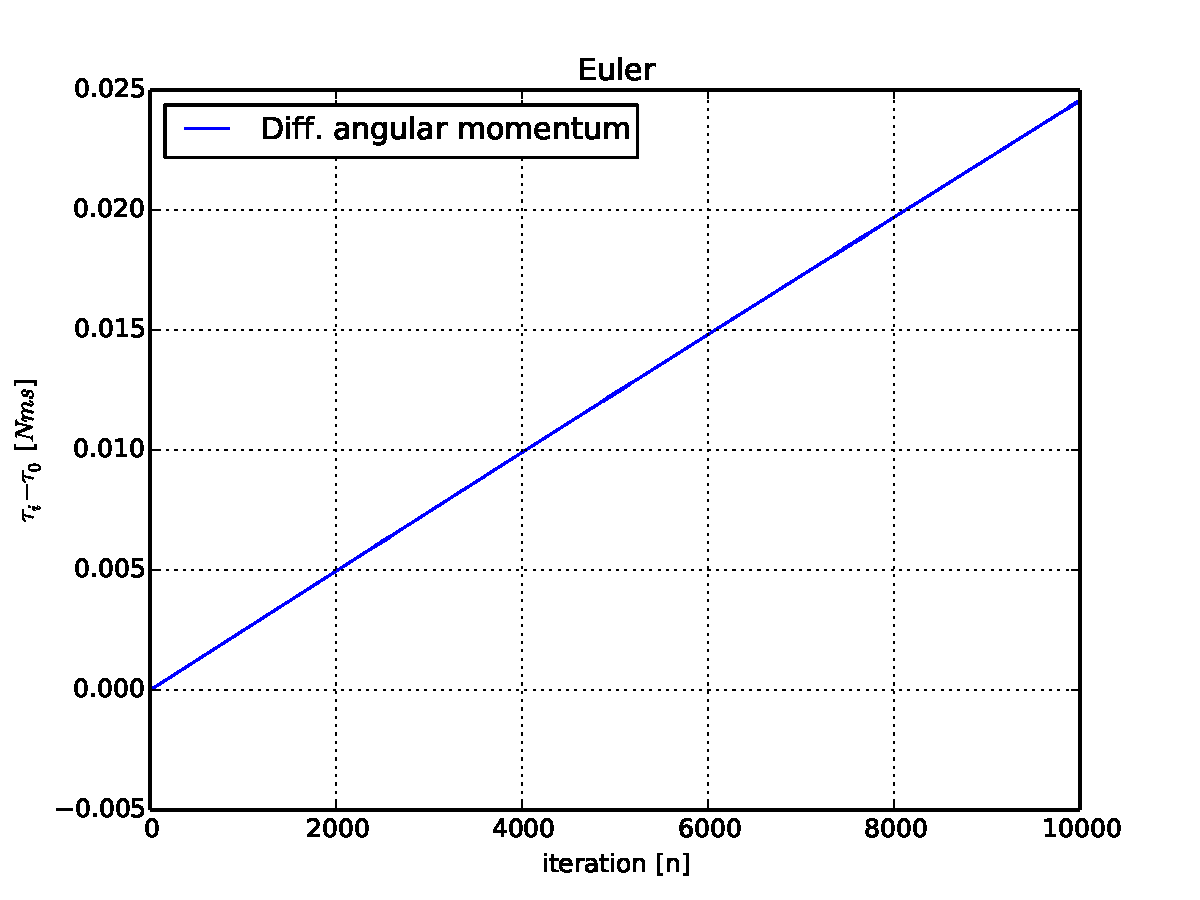
\includegraphics[width=\linewidth]{result/bilder/ang-momentum-euler.pdf}
        \caption{}
    \end{subfigure}%
    ~ 
    \begin{subfigure}{0.5\textwidth}
        \centering
        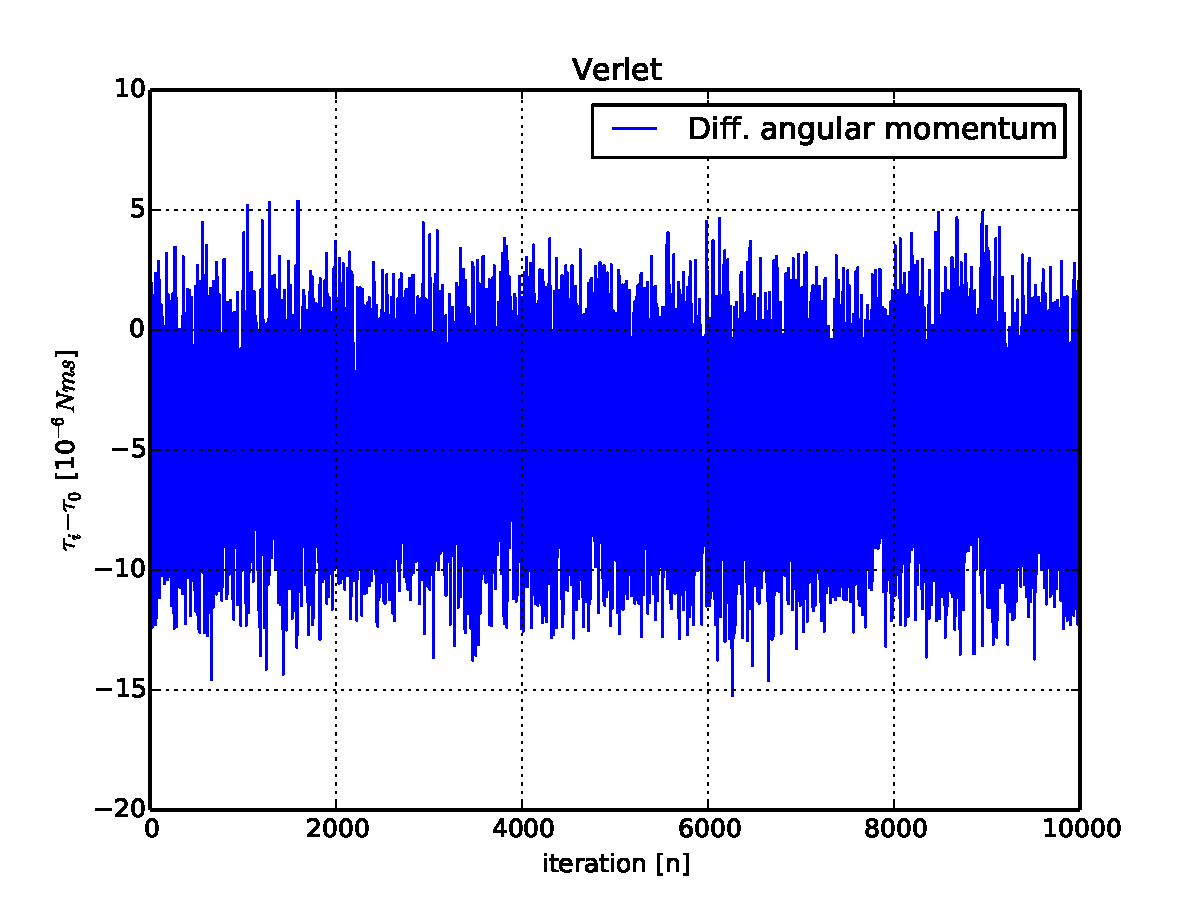
\includegraphics[width=\linewidth]{result/bilder/ang-momentum-verlet.pdf}
        \caption{}
    \end{subfigure}
    \caption{Both figures are graphs of the angular momentum and how they differ from their intial values. a) is the Forward Euler method and b) is the Verlet-Velocity method. 
    }
    \label{fig:conserved-ang}
\end{figure}

Forward Euler is once again not capable of conserving the value, but luckily for us the Verlet-Velocity method is. 













\subsubsection{Escape velocity}

The assignment was to find the escape velocity for the earth by trial and error. Fortunate for us that we know some math and can calculate it. See section \ref{sec:escape-velocity} for this. In practice this meant we started guessing "randomly" (winking Face emoji) before tuning the initial conditions to find the escape velocity. Figure (\ref{fig:escape-velocity-low}) a) shows these guesses where we can see that the velocities of around 8.8 au/yr causes the planet to shoot out and never return. 
The algorithms only runs for 15 years and will thereby not see the 8.8 au/year return to orbit even though it should. The plots were made by the data and python scripts in the directory \href{https://github.com/erikfsk/Project-3/tree/master/Project3/escape-velocity}{\textcolor{blue}{escape-velocity}}.

\begin{figure}[H]
    \centering
    \begin{subfigure}{0.5\textwidth}
        \centering
        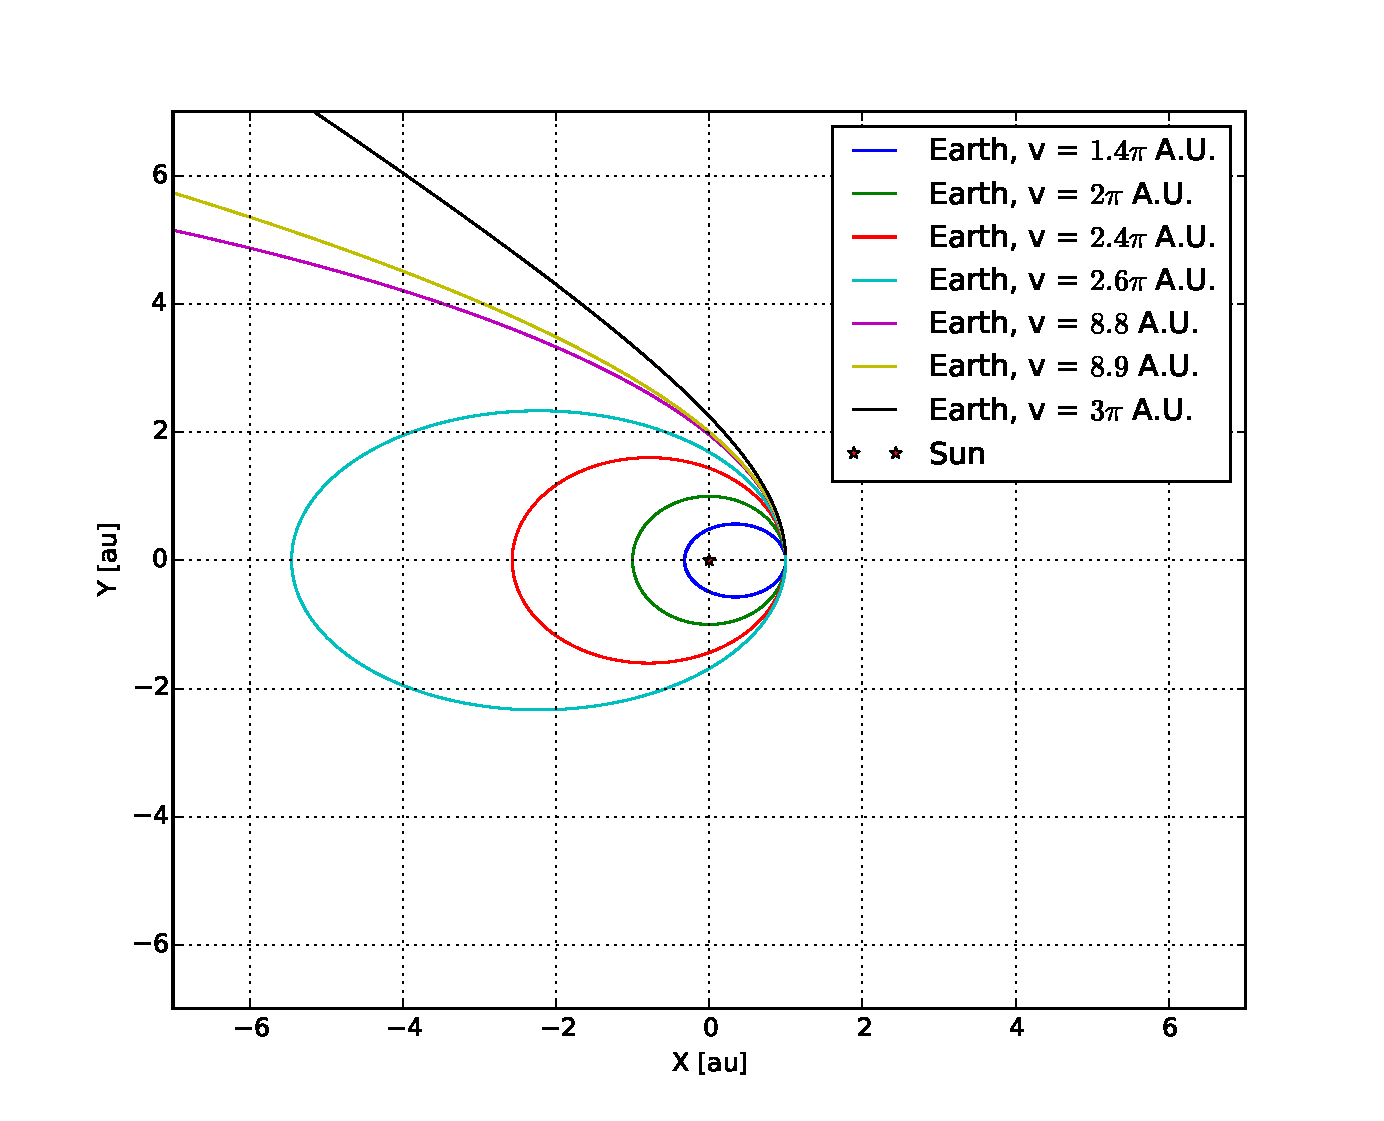
\includegraphics[width=\linewidth]{result/bilder/escape-velocity.pdf}
    	\caption{}
    \end{subfigure}%
    ~ 
    \begin{subfigure}{0.5\textwidth}
        \centering
        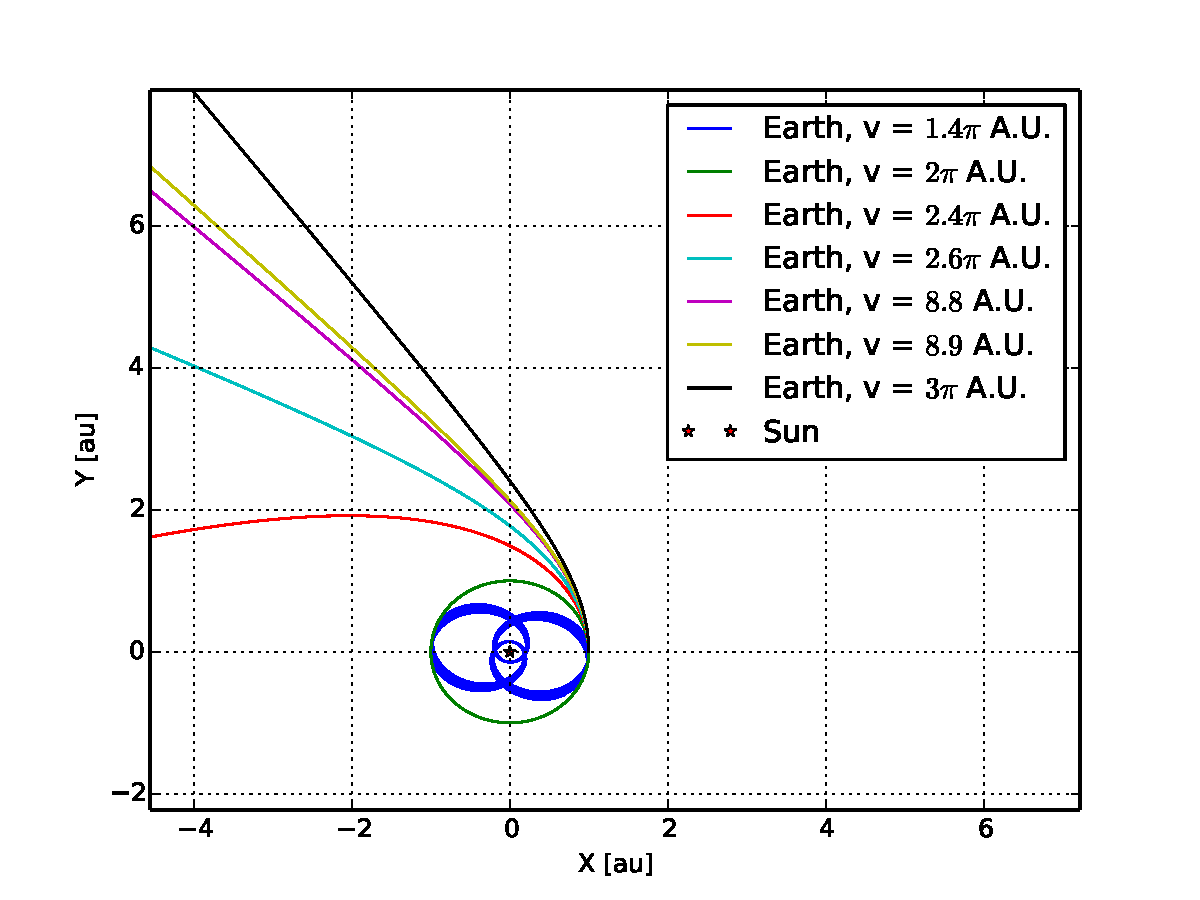
\includegraphics[width=\linewidth]{result/bilder/escape-velocity-r25.pdf}
        \caption{}
    \end{subfigure}
    \caption{a) Shows how the orbits of earths with different initial velocity develops. b) Shows the same as a) but this time the dependency of r in the denominator in equation (\ref{eq:newton}) is set to 3.5.}
    \label{fig:escape-velocity-low}
\end{figure}



\begin{figure}[H]
    \centering
    \begin{subfigure}{0.5\textwidth}
        \centering
        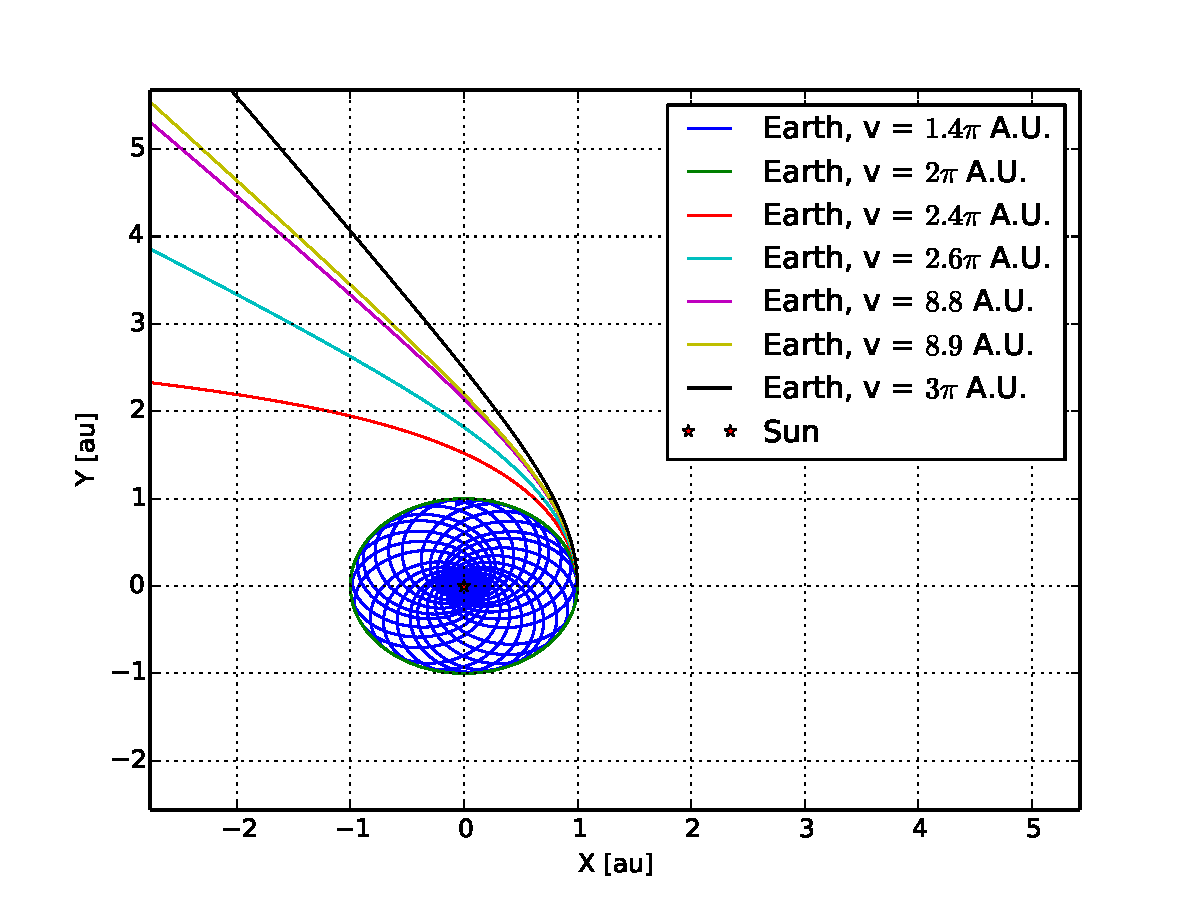
\includegraphics[width=\linewidth]{result/bilder/escape-velocity-r275.pdf}
    	\caption{}
    \end{subfigure}%
    ~ 
    \begin{subfigure}{0.5\textwidth}
        \centering
        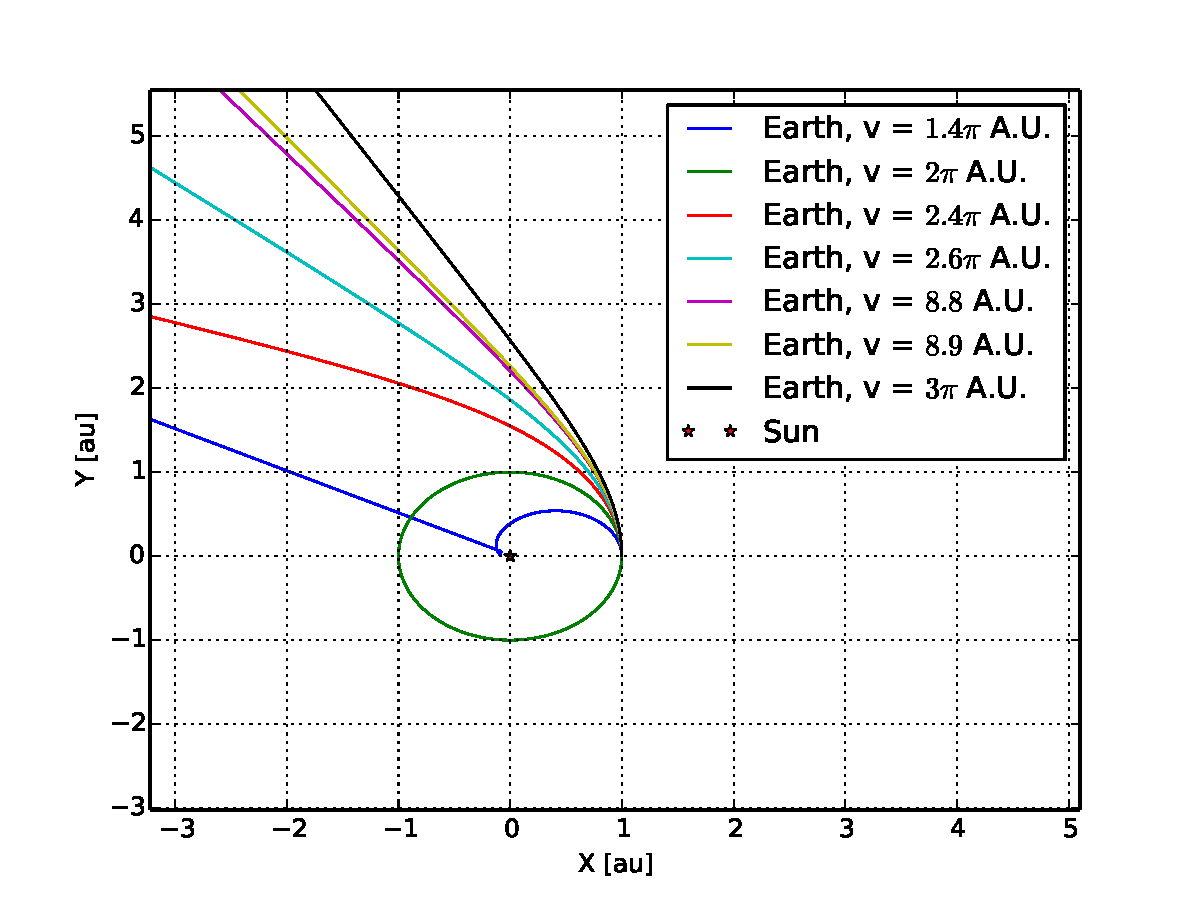
\includegraphics[width=\linewidth]{result/bilder/escape-velocity-r3.pdf}
        \caption{}
    \end{subfigure}
    \caption{a) Shows the same as figure (\ref{fig:escape-velocity-low}) but this time the dependency of r in the denominator in equation (\ref{eq:newton}) is set to 3.75. b) again shows the same as a) but now with the denominator set to 4.}
    \label{fig:escape-velocity-high}
\end{figure}


We are extremly lucky for living in a universe with a radius dependency of 2, but then again we probably would not exist if the dependency was different. All the other dependencies are very unstable for even the slightest change in velocity from the circular orbit velocity.


















\subsection{Three body system}

All the figures in this section has been made from the directory \href{https://github.com/erikfsk/Project-3/tree/master/Project3/mass%20jupitur}{\textcolor{blue}{mass jupitur}}. In this directory there are different directories for the r dependency and a python script to generate graphs. The effect of varying Jupiters mass was quite striking, as we saw in the simulations. Four different masses with factors of 10, 100, 1000 and 1100 was compared and can be seen in the plots below.

\subsubsection{Fixed mass for Jupitur}

For a simulation with Jupiters original mass $10^5$ points over 15 years is sufficient to calculate the orbits of the planets. Figure (\ref{fig:three-body}) is quite smooth and one should not expect to get any major change in the result even with many more points per year. 

\begin{figure}[H]
    \centering
    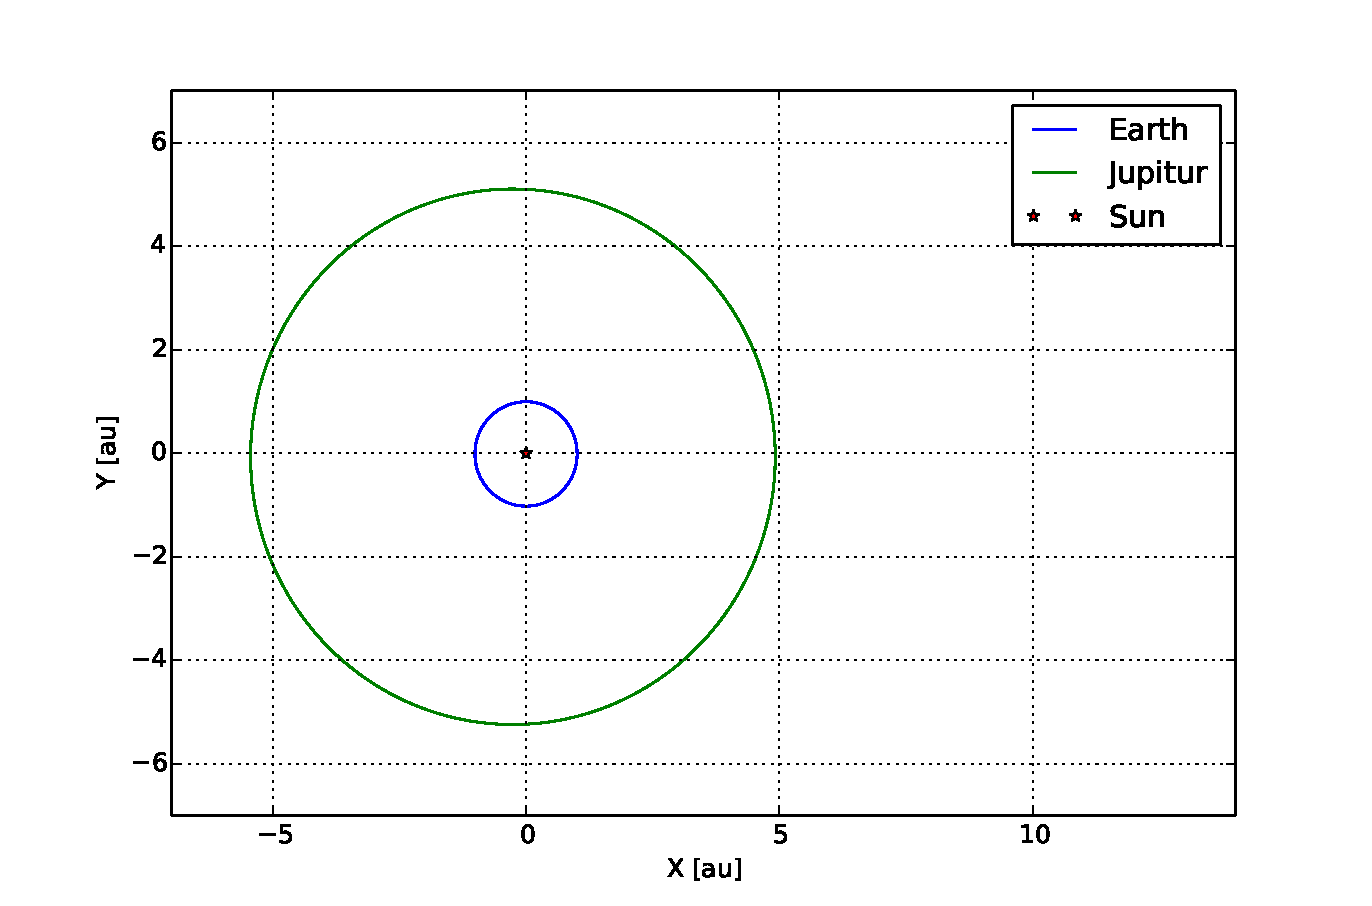
\includegraphics[width=\linewidth]{result/bilder/jupitur-mass.pdf}
    \caption{Plot of the three body system with Earth, Jupitur and the sun. n = 100000 over 15 years. The graph is discussed in the paragraph above. }
    \label{fig:three-body}
\end{figure}


\subsubsection{Varying mass for Jupiter}

For varying mass it is mostly the same as for the original mass. For the mass multiplied with 10 and 100 the orbit is normal with some slight changes and one should not expect any major differences with higher amount of points per year. For the biggest masses the results vary much more on the number of steps per year. We found that a couple of hundred thousand steps in total gave a good approximation. A bit higher step count makes earth disappear and a way bigger step count makes the earth come back to orbit like shown below. This is basicly the best of both worlds. The graphs has a relatively low amount of points, making it easier for the python plot, and has a pretty good approximation.

\begin{figure}[H]
    \centering
    \begin{subfigure}{0.5\textwidth}
        \centering
        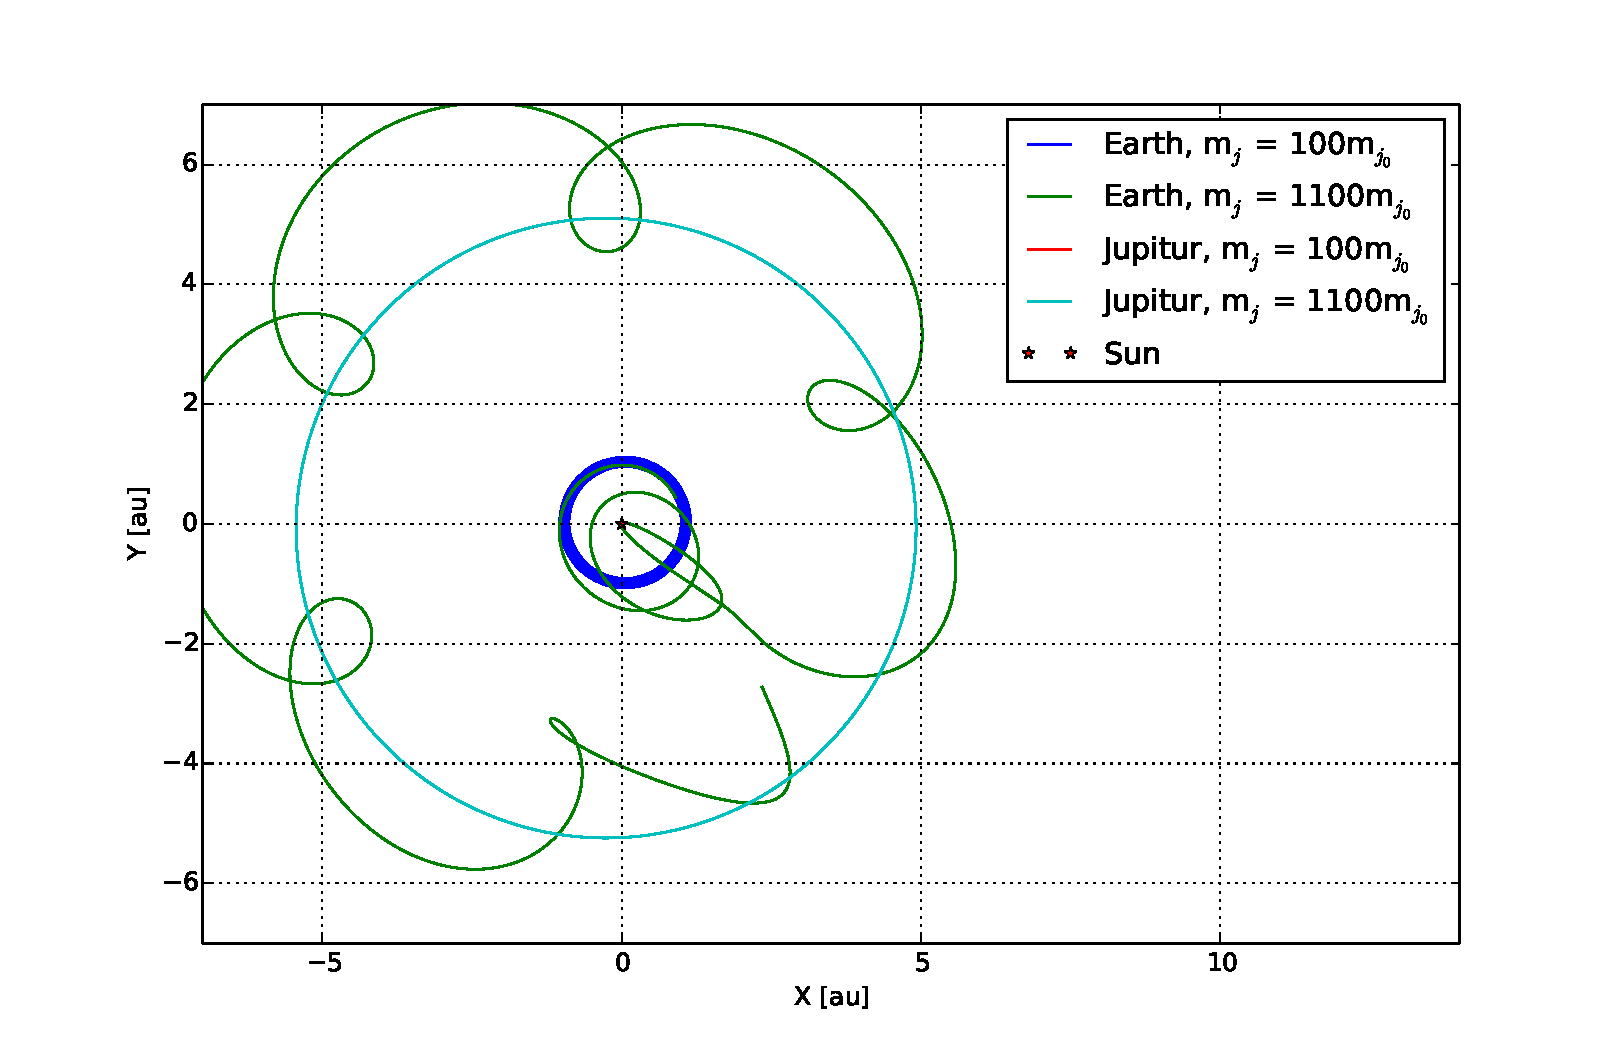
\includegraphics[width=\linewidth]{result/bilder/jupitur-mass-three.pdf}
    	\caption{}
    \end{subfigure}%
    ~ 
    \begin{subfigure}{0.5\textwidth}
        \centering
        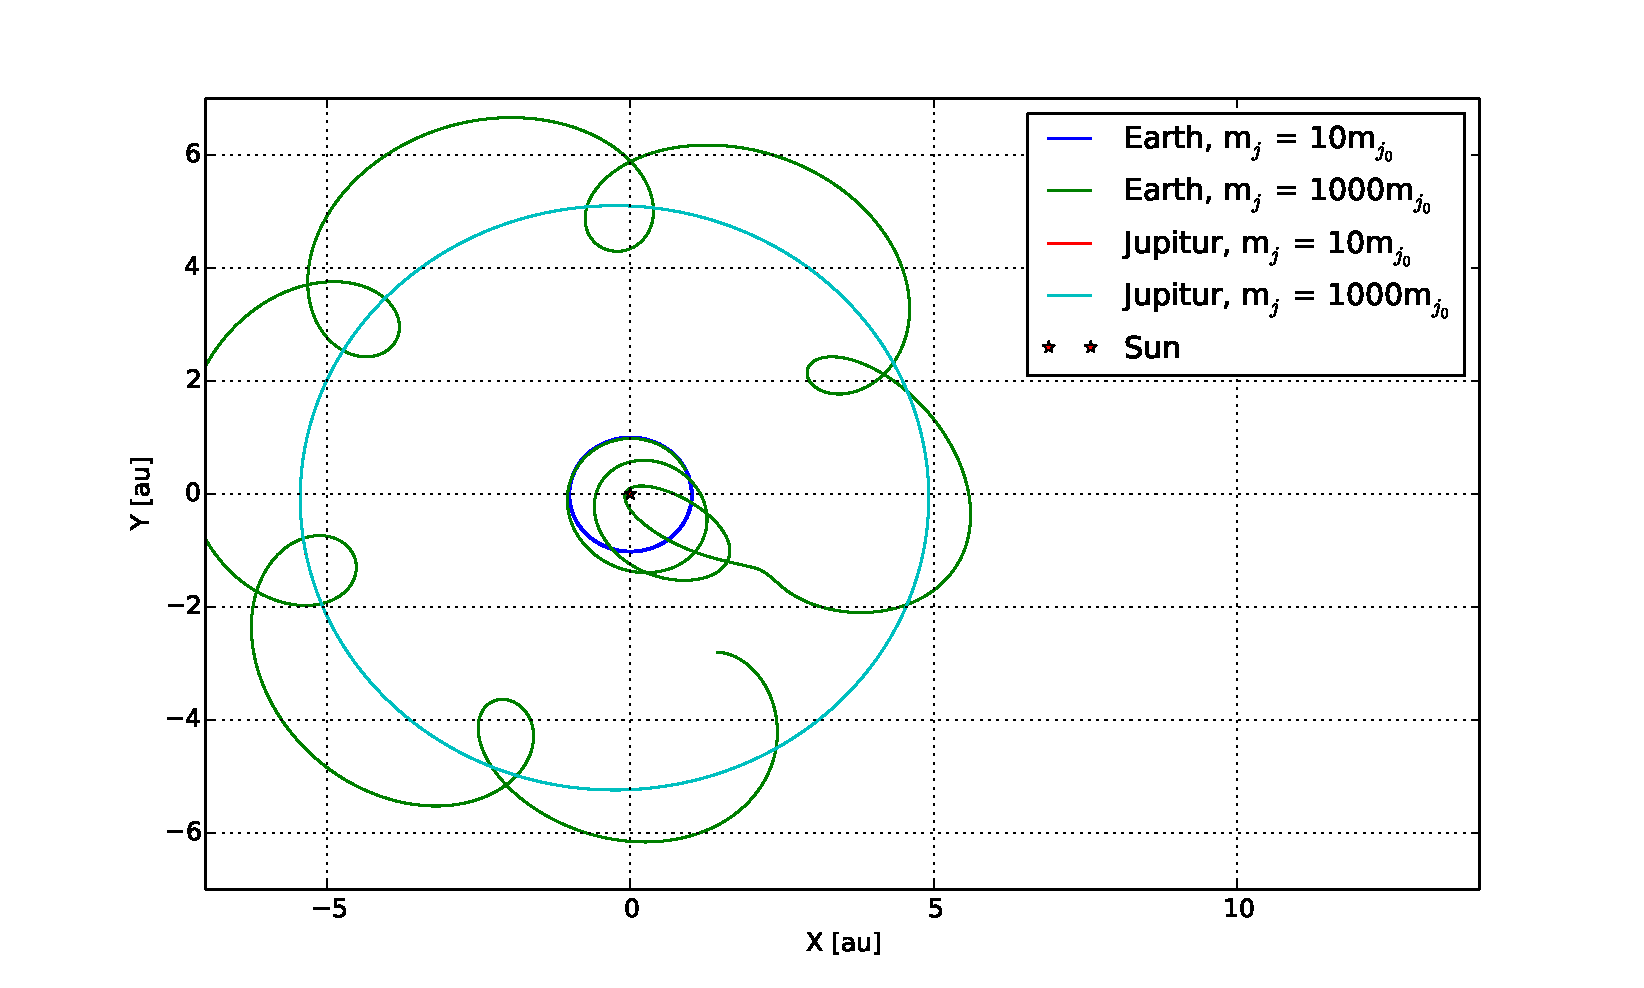
\includegraphics[width=\linewidth]{result/bilder/jupitur-mass-two.pdf}
        \caption{}
    \end{subfigure}
    \caption{Both plots has the sun as a fixed point. n = 100000 over 15 years. What the graphs represent is discussed above and legend should be pretty self explanatory.}
    \label{fig:three-body-varying}
\end{figure}











\subsection{Solar system}

All the figures in this section was made from the results and python scripts in the directory \href{https://github.com/erikfsk/Project-3/tree/master/Project3/full-solarsystem}{\textcolor{blue}{full-solarsystem}}.

\subsubsection{Three planets and all moving}

\begin{figure}[H]
    \centering
    \begin{subfigure}{0.5\textwidth}
        \centering
        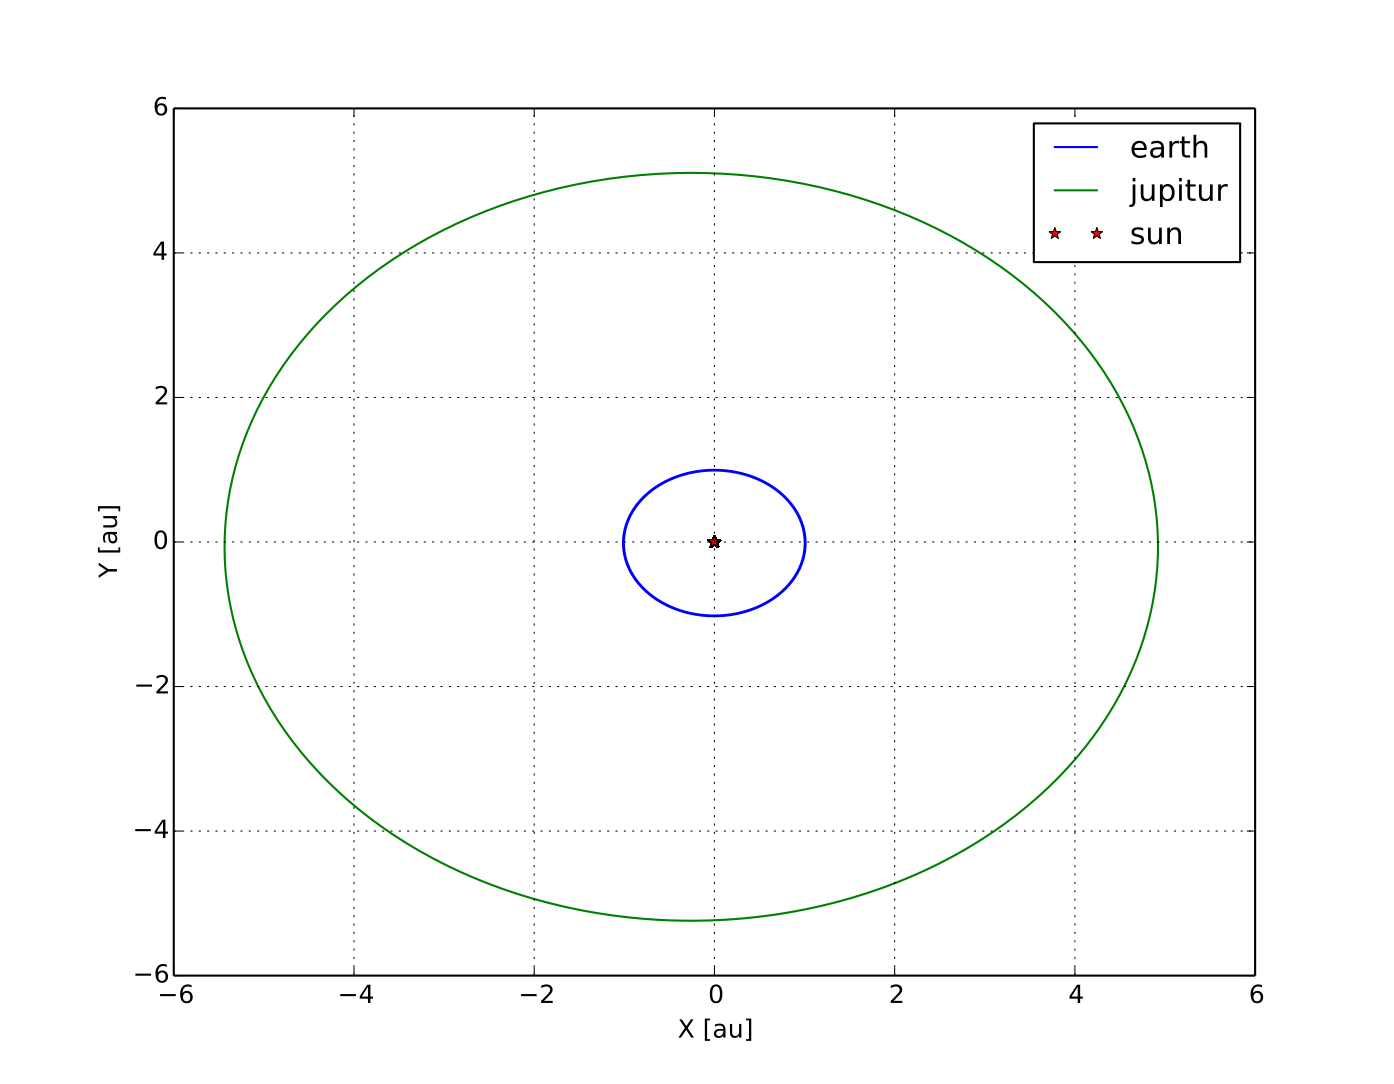
\includegraphics[width=\linewidth]{result/bilder/all-moving-jupitur.png}
        \caption{}
    \end{subfigure}%
    ~ 
    \begin{subfigure}{0.5\textwidth}
        \centering
        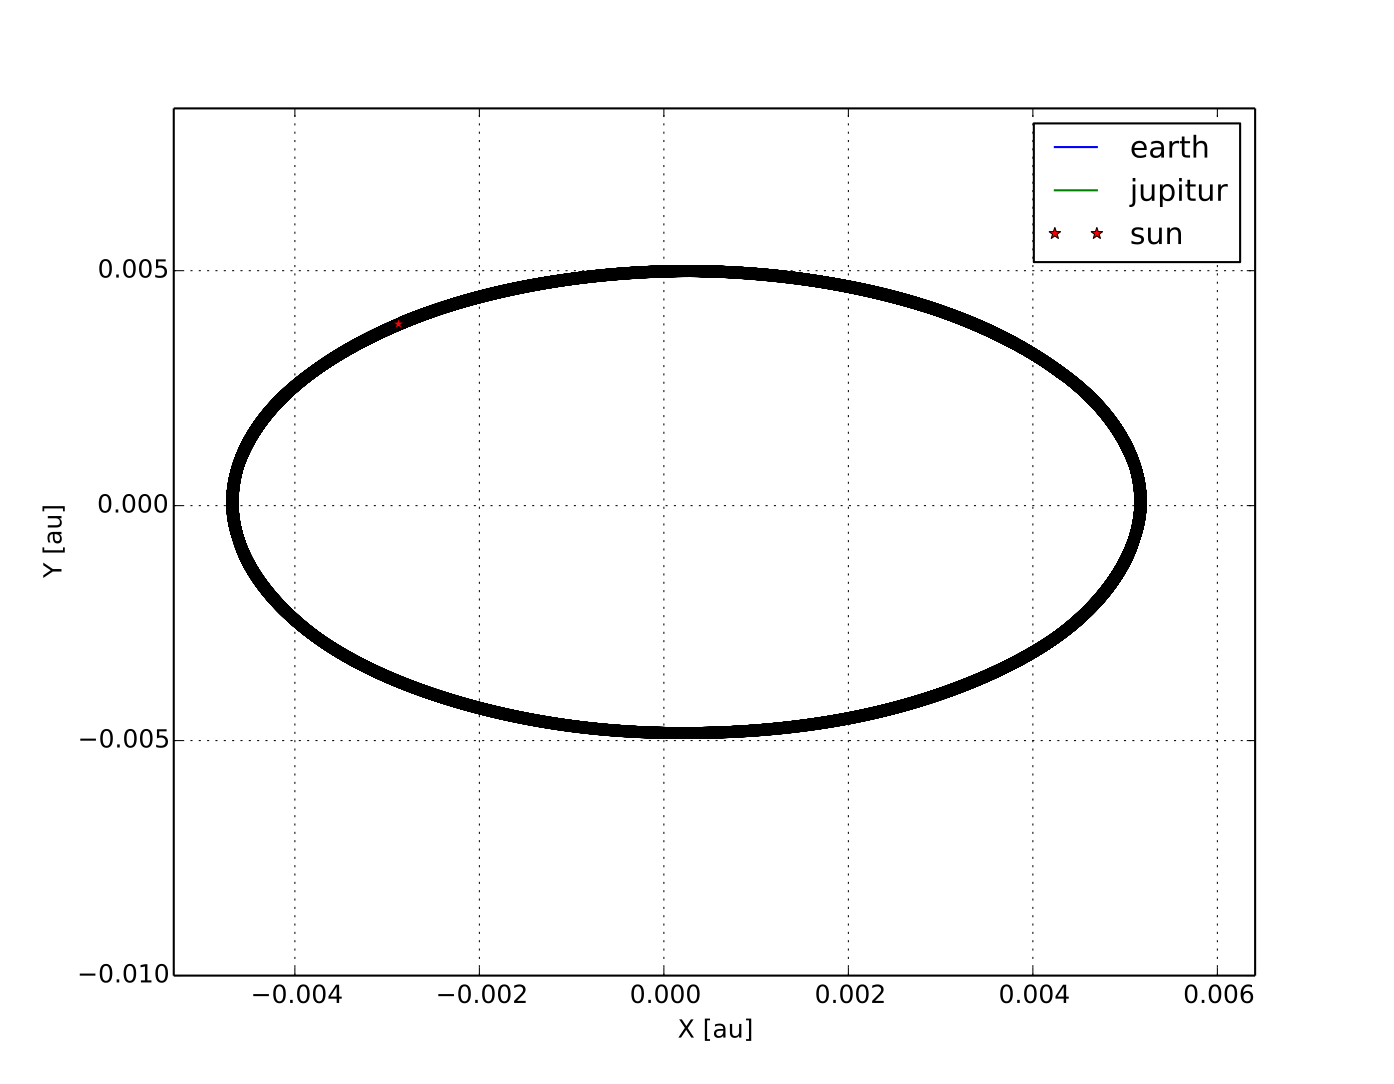
\includegraphics[width=\linewidth]{result/bilder/all-moving-jupitur-mass-center.png}
        \caption{}
    \end{subfigure}
    \caption{ n=$10^5$ and ran for 15 years. a) Shows the three body system solved with a moving sun. I b) is a zoom of the middle part of a). This is for verifying that the sun moves around the center of mass and is not drifting.}
    \label{fig:three-body-moving}
\end{figure}

The figure above has n=$10^5$ and ran for 15 years. If this would be used for any tests I would recommend using more points. To use more points here would be stupid. You can't see the difference.

\subsubsection{Solar system all moving}

\begin{figure}[H]
    \centering
    \begin{subfigure}{0.5\textwidth}
        \centering
        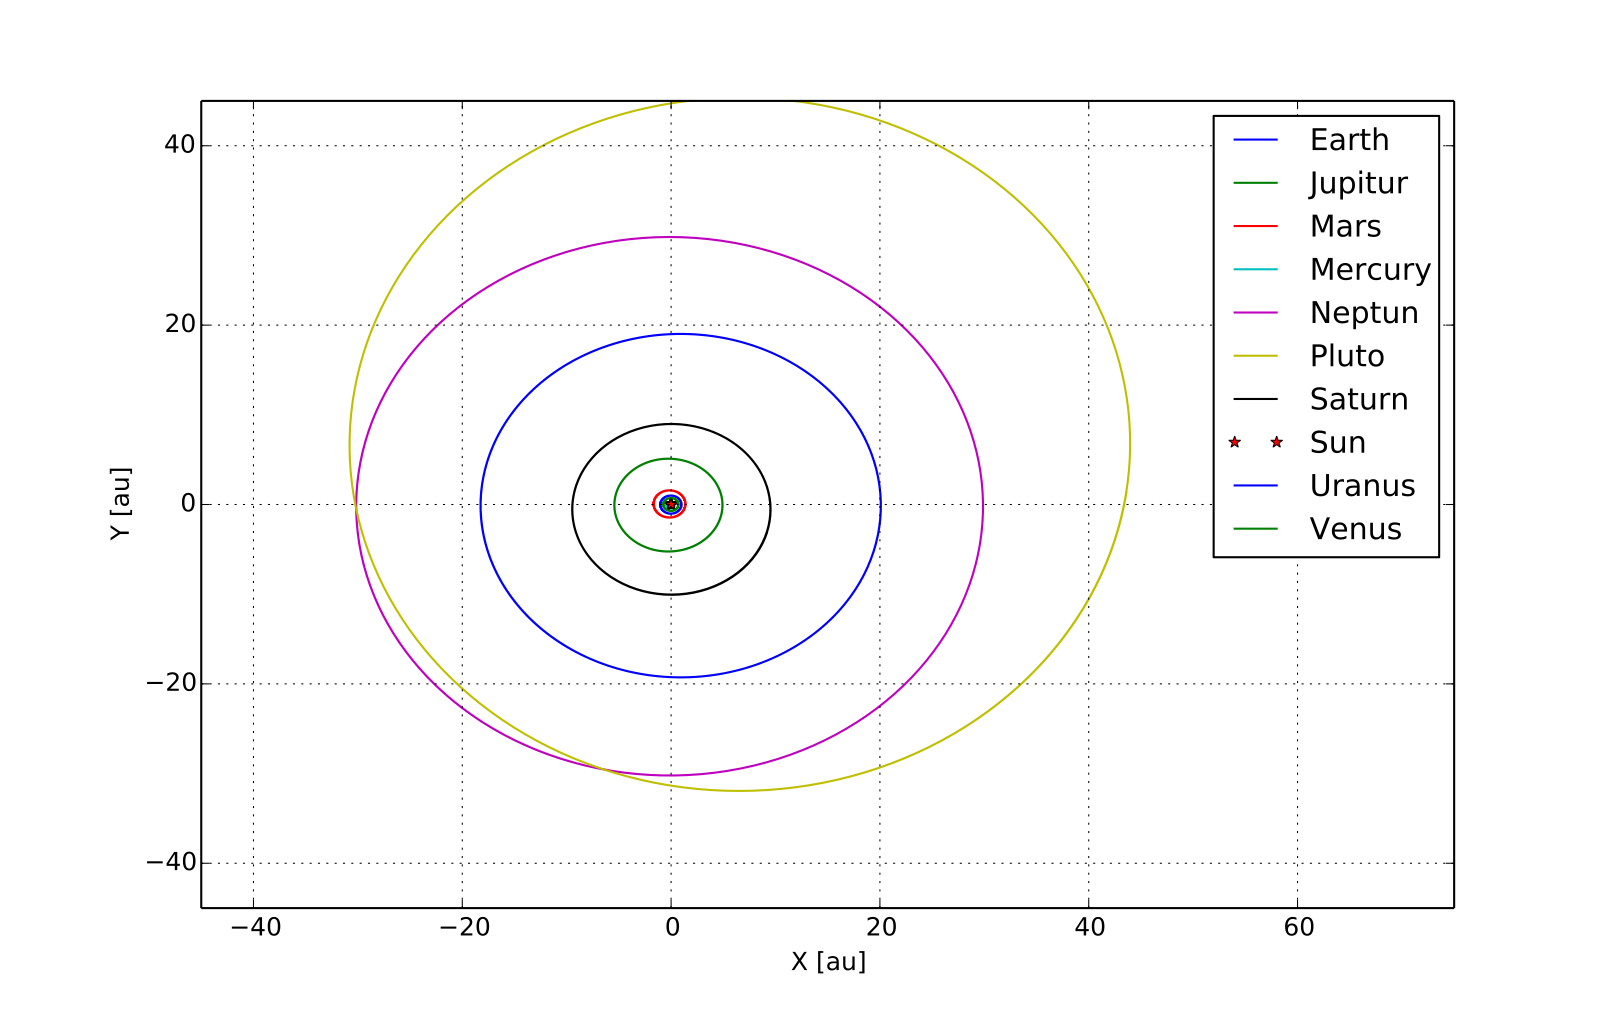
\includegraphics[width=\linewidth]{result/bilder/all-moving-solarsystem.png}
        \caption{}
    \end{subfigure}%
    ~ 
    \begin{subfigure}{0.5\textwidth}
        \centering
        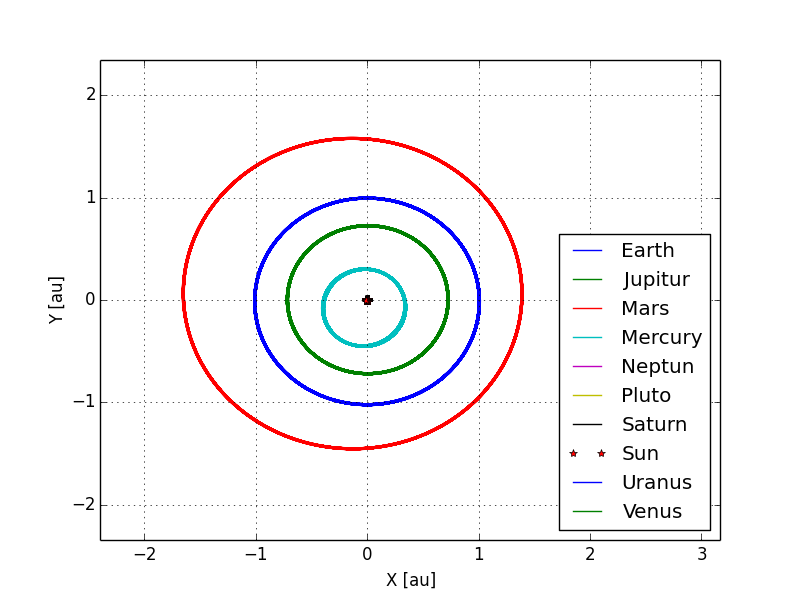
\includegraphics[width=\linewidth]{result/bilder/all-moving-solarsystem-zoom.png}
        \caption{}
    \end{subfigure}
    \caption{a) Shows the whole solar system solved with a moving sun.  b) is a zoom of the middle part of a). }
    \label{fig:solarsystem-moving}
\end{figure}

It has a n=$10^6$ and ran for 300 years. If this would be used for any tests I would recommend using more points, but this would be stupid for this figure, since you can't see the difference. Figure \ref{fig:solarsystem-moving} b) is for verifying that the sun also move in orbits around the center of mass, which is set to (0,0,0).


\pagebreak
\subsection{The perihelion precession of Mercury}

This has been discussed in section \ref{sec:perihelion}. The figure in this section was made from the results and python script in the directory \href{https://github.com/erikfsk/Project-3/tree/master/Project3/mercury-perihelion}{\textcolor{blue}{mercury-perihelion}}.


\begin{figure}[H]
    \centering
    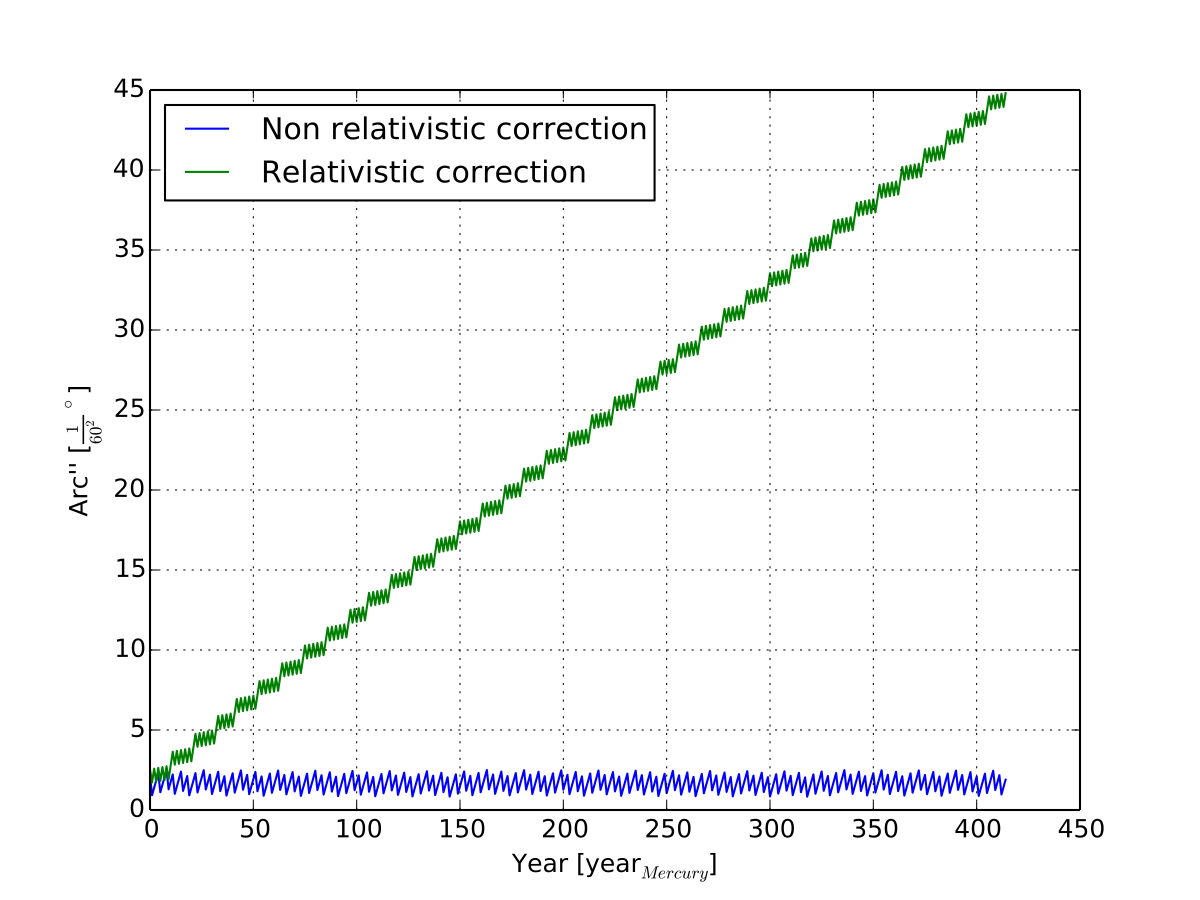
\includegraphics[width=0.8\linewidth]{result/bilder/perihelion.png}
    \caption{The graphs shows how Mercury orbit has moved in arc seconds as a function of orbits for Mercury.}
    \label{fig:perihelion}
\end{figure}

 After 100 years mercury perihelion should move about 43''. From the graphs we can see that it should move about 45''. This is probably due to numerical imprecision. The slopes inaccuracy is probably caused by the numerical solver precision. In other words more points would increase the accuracy. The jumping up and down along the linear curve is probably duo to the computer's accuracy with numbers. This will also improve by more steps, but one of them might stop to improve before the other.





